% Opening > Math 2.0
\section{Math 2.0}

% [1 min] Thesis, in Tao's terms. Left: Tao's 2x2 (AI use x human
% understanding). Right: Tao, with his "Math 2.0" quote. Bottom: the talk's
% thesis, boxed.
% The bracketed lead-in is an editorial paraphrase (Kyle), set in grey.
\begin{frame}{Math 1.0 and Math 2.0}
  \centering
  \begin{tikzpicture}[x=1cm, y=1cm]
    % bounding box = visible extent of the figure, so it centres in the body
    \useasboundingbox (0.1,0) rectangle (14.16,-6.45);
    % Tao's diagram
    \node[collagecard] at (3.75,-2.45) {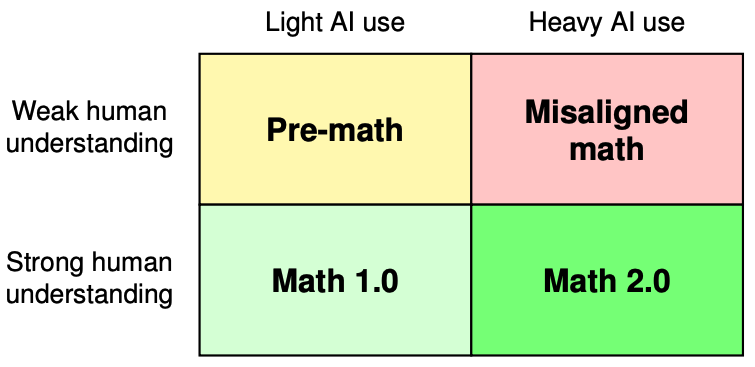
\includegraphics[width=6.8cm]{images/tao_math20.png}};
    % portrait, on a white disc with a soft shadow
    \node[circle, fill=white, inner sep=0pt, minimum size=2.02cm,
          drop shadow={shadow xshift=0.6pt, shadow yshift=-0.8pt, opacity=0.25}] at (11.3,-1.03) {};
    \node at (11.3,-1.03) {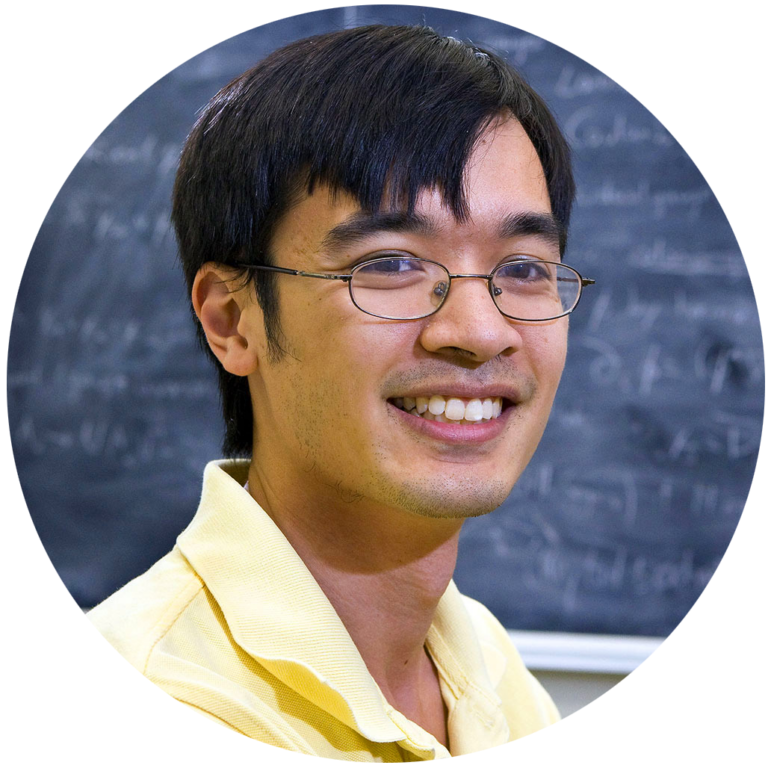
\includegraphics[width=1.92cm]{images/terry_tao.png}};
    % quote
    \node[anchor=north, text width=5.6cm, align=flush left, inner sep=0pt,
          font=\rmfamily\itshape\footnotesize] (q) at (11.35,-2.35)
      {{\color{black!50}\upshape[}{\color{black!55}Rather than blindly using AI to generate misaligned mathematics,}{\color{black!50}\upshape]}
       the more sustainable \textup{``Math 2.0''} use of AI would be to strengthen all the ways in which
       human understanding interacts with mathematics.};
    \node[anchor=north east, inner sep=0pt, font=\rmfamily\fontsize{26}{26}\selectfont, text=PennRed!80]
      at ([xshift=-0.05cm, yshift=0.12cm]q.north west) {``};
    % attribution
    \node[anchor=north west, inner sep=0pt, font=\sffamily\scriptsize, text=black!60, text width=6.0cm, align=left]
      at ([yshift=-0.22cm]q.south west)
      {--- Terence Tao, \emph{Machine Assisted Proof},\\AIM Public Lecture, Caltech, 9 Oct 2026};
    % thesis
    \node[anchor=south, draw=PennBlue!55, fill=PennBlue!4, line width=0.6pt, rounded corners=2pt,
          text width=11.4cm, inner xsep=0.3cm, inner ysep=0.2cm, align=left, font=\sffamily\small]
      at (7.13,-6.45)
      {\emph{
          For mathematicians, theorists, and theoretically-inclined experimentalists alike, gracefully and ethically navigating the transition to Math 2.0 will require reckoning with societal-level issues as well as developing individual familiarity with the emergent paradigm of AI-assisted formalization.
      %   Gracefully navigating the transition to Math~2.0 requires
      %  reckoning with societal level issues as well as understanding emerging best practices to capitalize
      %  on AI-driven workflows while maintaining scientific integrity, foremost by the principled integration of autoformalization into the theorists toolbox.
       }};
  \end{tikzpicture}
  \slidesources{Quote and diagram: T.~Tao, \emph{Machine Assisted Proof}, AIM Public Lecture Series, Caltech, 9 Oct 2026 (caltech.edu/campus-life-events/calendar/aim-public-lecture-series-terence-tao-1)}
\end{frame}

% [0.5 min] Overview: one card per part, listing that part's sections. The
% lists are generated from the section tree (\tableofcontents, subsections
% hidden), so they follow any change to the structure in main.tex.
% Beamer numbers the parts 1--4, so Part I is part=2 and Part II is part=3.
{
\setbeamertemplate{section in toc}{%
  \leavevmode\hbox to 0.9em{\color{PennRed}\rule[0.18ex]{0.42em}{0.42em}\hfil}%
  \inserttocsection\par}
\setbeamercolor{section in toc}{fg=black!80}
\newcommand{\overviewcard}[3]{% #1 label, #2 part name, #3 part number in the toc
  \begin{tikzpicture}[x=1cm, y=1cm, baseline={(0,0)}]
    \def\w{6.6}\def\h{4.4}\def\hb{1.25}
    \useasboundingbox (0,0) rectangle (\w,-\h);
    % card
    \fill[white, rounded corners=3pt,
          drop shadow={shadow xshift=0.6pt, shadow yshift=-0.8pt, opacity=0.25}] (0,0) rectangle (\w,-\h);
    % header band
    \begin{scope}
      \clip[rounded corners=3pt] (0,0) rectangle (\w,-\h);
      \fill[PennBlue] (0,0) rectangle (\w,-\hb);
      \fill[PennRed] (0,-\hb) rectangle (\w,{-\hb-0.06});
    \end{scope}
    \draw[black!15, line width=0.4pt, rounded corners=3pt] (0,0) rectangle (\w,-\h);
    \node[anchor=south west, inner sep=0pt, font=\sffamily\scriptsize\bfseries, text=white!70!PennBlue]
      at (0.45,-0.52) {\MakeUppercase{#1}};
    \node[anchor=north west, inner sep=0pt, font=\sffamily\Large, text=white]
      at (0.45,-0.6) {#2};
    % sections of this part
    \node[anchor=north west, inner sep=0pt, text width={\w cm - 0.9cm}, font=\sffamily\normalsize]
      at (0.45,{-\hb-0.05}) {\tableofcontents[part=#3, hideallsubsections]};
  \end{tikzpicture}%
}
\begin{frame}{The rest of this talk}
  \vspace*{0.87cm}
  \centering
  \overviewcard{Part I}{\partnameone}{2}\hspace{0.7cm}%
  \overviewcard{Part II}{\partnametwo}{3}
\end{frame}
}

